% =====================================================================
% Kapitel 7: Notebook-Generator
% =====================================================================

\chapter{Notebook-Generator}

\label{ch:notebook}

Das \emph{Jupyter-Notebook} ist die komfortabelste Form, um
Finanzmarktdaten zu visualisieren. Es ermöglicht interaktive
Charts, schrittweises Erforschen und einfaches Teilen der Ergebnisse
als HTML.

\section{Überblick: Pipeline}

\begin{figure}[ht]
\centering
\begin{tikzpicture}[
  node distance=0.8cm and 1.2cm,
  box/.style={rectangle, draw, thick, rounded corners, minimum width=2.5cm, minimum height=0.8cm, align=center, font=\small},
  file/.style={ellipse, draw, thick, minimum width=2.5cm, font=\small, align=center},
  arrow/.style={-Latex, thick},
]
  \node[file, fill=cyan!20] (build) {build\_notebook.py};
  \node[file, fill=yellow!20, right=of build] (ipynb) {\code{01\_macro\_overview.ipynb}};
  \node[file, fill=green!20, right=of ipynb] (html) {\code{01\_macro\_overview.html}};

  \draw[arrow] (build) -- node[above, font=\scriptsize] {\code{nbformat}} (ipynb);
  \draw[arrow] (ipynb) -- node[above, font=\scriptsize] {\code{nbconvert --execute}} (html);
\end{tikzpicture}
\caption{Build-Pipeline für das Notebook. \code{build\_notebook.py}
  erzeugt die \code{.ipynb} programmatisch aus Cell-Definitionen.
  \code{jupyter nbconvert} führt die Cells aus und exportiert HTML.}
\label{fig:notebook-pipeline}
\end{figure}

\section{Warum programmatisch generieren?}

\begin{warnung}
\rmfamily\itshape
\foreign{Notebook-Ausführungs-Ausgaben veralten schnell}. Wenn ein
Notebook committet wird, sind die eingebetteten Plots und Tabellen
\emph{für immer} eingefroren -- egal, wie sich die Daten dahinter
ändern. Das führt zu \emph{stale-notebooks}, in denen der Leser
nicht erkennt, dass die Daten veraltet sind.
\end{warnung}

Die Lösung: \emph{Trennung} zwischen \code{Quellcode} (Cell-Definitionen
in Python) und \emph{Output} (gerendertes Notebook + HTML). Die
\code{.ipynb}-Datei ist ein \emph{Build-Artefakt}, das jederzeit
regeneriert werden kann.

\section{Der Build-Prozess}

Listing~\ref{lst:build} zeigt das Herzstück von
\code{scripts/build\_notebook.py}.

\begin{lstlisting}[language=python, caption={Notebook programmatisch erzeugen},label=lst:build]
import nbformat as nbf

CELLS = [
    nbf.v4.new_markdown_cell("# deephold_db — Macro Overview"),
    nbf.v4.new_code_cell("from deephold_db.db import session_scope, MacroObservation"),
    nbf.v4.new_code_cell("..."),
    nbf.v4.new_markdown_cell("## Plots"),
    nbf.v4.new_code_cell("fig = make_subplots(...)"),
    nbf.v4.new_code_cell("fig.show()"),
    nbf.v4.new_markdown_cell("## Summary"),
    nbf.v4.new_code_cell("summary = pl.DataFrame(rows); print(summary)"),
]

def main():
    nb = nbf.v4.new_notebook()
    nb.cells = CELLS
    nb.metadata = {"kernelspec": {"name": "python3"}}
    nbf.write(nb, NOTEBOOK_PATH)
    subprocess.run(["jupyter", "nbconvert", "--execute", "--inplace", str(NOTEBOOK_PATH)])
    subprocess.run(["jupyter", "nbconvert", "--to", "html", str(NOTEBOOK_PATH)])
\end{lstlisting}

Der Build-Prozess ist in vier Schritte:

\begin{enumerate}
  \item \textbf{Cell-Definition}: Python-Liste von
        \code{nbf.v4.new\_markdown\_cell()} und
        \code{nbf.v4.new\_code\_cell()} Objekten.
  \item \textbf{Notebook schreiben}: \code{nbf.write()} erzeugt
        eine valides \code{.ipynb}-JSON-Datei.
  \item \textbf{Execute}: \code{jupyter nbconvert --execute}
        führt alle Code-Cells aus und bettet die Outputs in die
        \code{.ipynb} ein.
  \item \textbf{Export}: \code{jupyter nbconvert --to html}
        erzeugt eine statische HTML-Datei, die ohne Jupyter
        geöffnet werden kann.
\end{enumerate}

\section{Plotly 3$\times$2-Grid}

Das Notebook zeigt 6~Subplots in einem 3$\times$2-Grid
(Abbildung~\ref{fig:notebook-grid}):

\begin{figure}[ht]
\centering
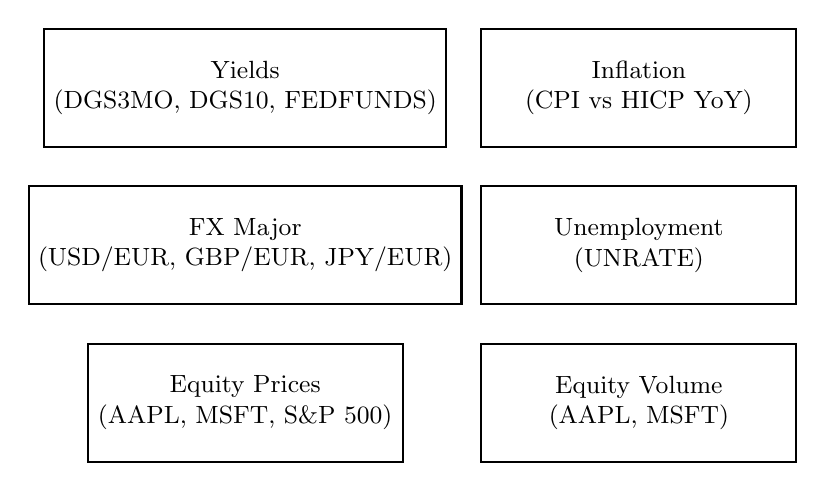
\begin{tikzpicture}[
  box/.style={rectangle, draw, thick, minimum width=4cm, minimum height=1.5cm, align=center, font=\small},
  arrow/.style={-Latex, thick},
]
  \node[box] (y) at (0, 2) {Yields\\(DGS3MO, DGS10, FEDFUNDS)};
  \node[box] (i) at (5, 2) {Inflation\\(CPI vs HICP YoY)};
  \node[box] (fx) at (0, 0) {FX Major\\(USD/EUR, GBP/EUR, JPY/EUR)};
  \node[box] (un) at (5, 0) {Unemployment\\(UNRATE)};
  \node[box] (ep) at (0, -2) {Equity Prices\\(AAPL, MSFT, S\&P 500)};
  \node[box] (ev) at (5, -2) {Equity Volume\\(AAPL, MSFT)};
\end{tikzpicture}
\caption{3$\times$2 Plotly-Subplot-Grid im Notebook. Die obere
  Hälfte zeigt Makro-Daten, die untere Hälfte Equity-Daten.}
\label{fig:notebook-grid}
\end{figure}

Jeder Subplot hat seine eigenen \emph{Y-Achsen-Skalen}, weil die
Größenordnungen fundamental verschieden sind (Zinssätze in
\,\%, Aktienkurse in USD, Volumen in Milliarden).

\section{HTML-Export}

Der HTML-Export hat zwei Verwendungszwecke:

\begin{itemize}
  \item \textbf{Sharing}: Man kann die HTML-Datei per Mail
        verschicken oder auf einem Webserver ablegen, ohne dass
        der Empfänger Jupyter installieren muss.
  \item \textbf{Caching}: Die HTML-Datei ist ein \emph{Snapshot}
        der Daten zum Build-Zeitpunkt. Wenn die DB später
        aktualisiert wird, bleibt der HTML-Snapshot konsistent.
\end{itemize}

\begin{merke}
Die HTML-Datei \emph{referenziert} plotly.js von einem CDN. Ohne
Internet-Zugang beim Öffnen der HTML-Datei sind die Plots
\emph{nicht} sichtbar -- die zugrundeliegenden Daten sind aber
weiterhin im HTML-Markup eingebettet.
\end{merke}

\section{Was als Nächstes?}

Das Notebook ist eine schöne \emph{Passive-View} der Daten. Für
\emph{aktive Exploration} -- Springen zwischen Serien, Suche,
Keyboard-Navigation -- brauchen wir etwas anderes: das
\emph{OpenTUI-Explorer}, das im nächsten Kapitel vorgestellt wird.
